\pagebreak


\section*{Q2}
\begin{solution}[\textbf{2}]
\hfill\break
Code is given in separate file. The convergence table for the three methods with initial condition 
\begin{align*}
 u(x,0) = \sin(\pi x)
\end{align*}
is given by,
\begin{figure}[H]
    \centering
    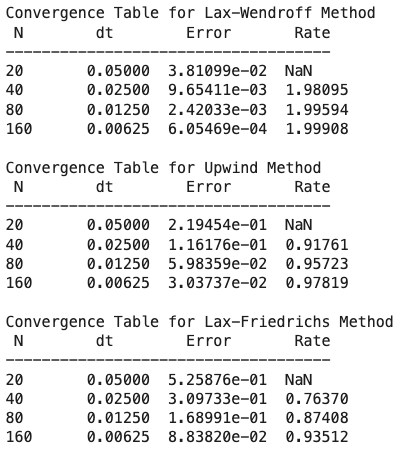
\includegraphics[scale=0.5]{./figures/q2-table.png}
\end{figure}
We see Upwind and Lax-Friedrichs method converge to $1$ as we expect, similarly Lax-Wendroff converges to $2$ as we expect.
\end{solution}

